% Chapter 4, Section 2: Gradient-Based Optimization

\section{Gradient-Based Optimization \difficultyInline{beginner}}
\label{sec:gradient-optimization}

\subsection{Intuition: Finding the Bottom of a Hill}

Imagine you're hiking in foggy mountains and need to find the lowest point in a valley. You can't see far ahead, but you can feel the slope under your feet. The steepest downward direction tells you which way to walk to get lower.

This is exactly what gradient descent does:
\begin{itemize}
    \item \textbf{The mountain} = the loss function we want to minimize
    \item \textbf{Your position} = current parameter values
    \item \textbf{The slope} = gradient (direction of steepest increase)
    \item \textbf{Your steps} = parameter updates
\end{itemize}

Most deep learning algorithms involve optimization: finding parameters that minimize or maximize an objective function.

\subsection{Gradient Descent}

For a function $f(\vect{\theta})$, \textbf{gradient descent} updates parameters as:

\begin{equation}
\vect{\theta}_{t+1} = \vect{\theta}_t - \alpha \nabla_{\vect{\theta}} f(\vect{\theta}_t)
\end{equation}

where $\alpha > 0$ is the \textbf{learning rate}.

\subsubsection{Example: Gradient Descent in 2D}

Consider minimizing $f(x, y) = x^2 + 2y^2$ starting from $(3, 3)$:

\begin{figure}[h]
\centering
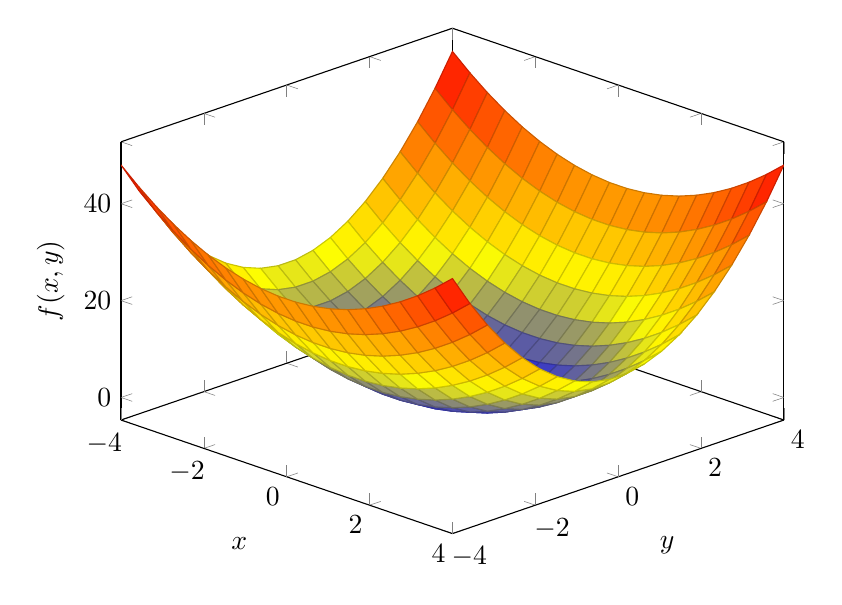
\begin{tikzpicture}
\begin{axis}[
    xlabel={$x$},
    ylabel={$y$},
    zlabel={$f(x,y)$},
    width=10cm,
    height=8cm,
    view={45}{30}
]
\addplot3[
    surf,
    domain=-4:4,
    domain y=-4:4,
    samples=20
] {x^2 + 2*y^2};
\end{axis}
\end{tikzpicture}
\caption{Contour plot of $f(x,y) = x^2 + 2y^2$ showing gradient descent path}
\label{fig:gradient-descent-2d}
\end{figure}

The gradient is $\nabla f = [2x, 4y]$. Starting from $(3, 3)$ with learning rate $\alpha = 0.1$:
\begin{align}
\nabla f(3, 3) &= [6, 12] \\
(x_1, y_1) &= (3, 3) - 0.1[6, 12] = (2.4, 1.8) \\
\nabla f(2.4, 1.8) &= [4.8, 7.2] \\
(x_2, y_2) &= (2.4, 1.8) - 0.1[4.8, 7.2] = (1.92, 1.08)
\end{align}

\subsection{Jacobian and Hessian Matrices}

The \textbf{Jacobian matrix} contains all first-order partial derivatives. For $\vect{f}: \mathbb{R}^n \to \mathbb{R}^m$:

\begin{equation}
\mat{J}_{ij} = \frac{\partial f_i}{\partial x_j}
\end{equation}

The \textbf{Hessian matrix} contains second-order derivatives:

\begin{equation}
\mat{H}_{ij} = \frac{\partial^2 f}{\partial x_i \partial x_j}
\end{equation}

The Hessian characterizes the local curvature of the function.

\subsection{Taylor Series Approximation}

Near point $\vect{x}_0$, we can approximate $f(\vect{x})$ using Taylor series:

\begin{equation}
f(\vect{x}) \approx f(\vect{x}_0) + (\vect{x} - \vect{x}_0)^\top \nabla f(\vect{x}_0) + \frac{1}{2}(\vect{x} - \vect{x}_0)^\top \mat{H}(\vect{x}_0) (\vect{x} - \vect{x}_0)
\end{equation}

This provides insight into optimization behavior.

\subsection{Critical Points}

\subsubsection{Intuition: Different Types of Critical Points}

Think of critical points as different types of terrain features:

\begin{itemize}
    \item \textbf{Local minimum} = Bottom of a bowl - you can't go lower in any direction
    \item \textbf{Local maximum} = Top of a hill - you can't go higher in any direction  
    \item \textbf{Saddle point} = Mountain pass - you can go down in some directions, up in others
\end{itemize}

At a \textbf{critical point}, $\nabla f(\vect{x}) = \boldsymbol{0}$. The Hessian determines the nature:
\begin{itemize}
    \item \textbf{Local minimum:} Hessian is positive definite
    \item \textbf{Local maximum:} Hessian is negative definite
    \item \textbf{Saddle point:} Hessian has both positive and negative eigenvalues
\end{itemize}

\begin{figure}[h]
\centering
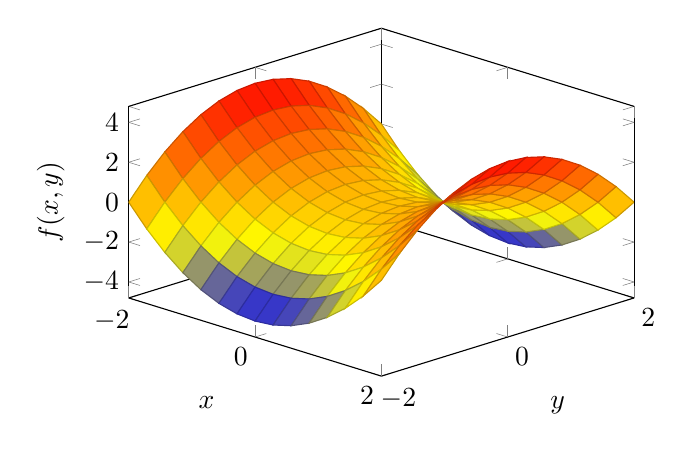
\begin{tikzpicture}
\begin{axis}[
    xlabel={$x$},
    ylabel={$y$},
    zlabel={$f(x,y)$},
    width=8cm,
    height=6cm,
    view={45}{30}
]
\addplot3[
    surf,
    domain=-2:2,
    domain y=-2:2,
    samples=15
] {x^2 - y^2};
\end{axis}
\end{tikzpicture}
\caption{Example of a saddle point: $f(x,y) = x^2 - y^2$}
\label{fig:saddle-point}
\end{figure}

Deep learning often encounters saddle points rather than local minima in high dimensions.

\subsection{Directional Derivatives}

The directional derivative in direction $\vect{u}$ (with $\|\vect{u}\| = 1$) is:

\begin{equation}
\frac{\partial}{\partial \alpha} f(\vect{x} + \alpha \vect{u}) \bigg|_{\alpha=0} = \vect{u}^\top \nabla f(\vect{x})
\end{equation}

To minimize $f$, we move in the direction $\vect{u} = -\frac{\nabla f(\vect{x})}{\|\nabla f(\vect{x})\|}$.
